% Documents setup
\documentclass[11pt]{book}

% fix for pandoc 1.14
\providecommand{\tightlist}{%
  \setlength{\itemsep}{0pt}\setlength{\parskip}{0pt}}

\usepackage{tabu} % https://tex.stackexchange.com/questions/50332/vertical-spacing-of-a-table-cell

% Location of the csas-style repository: adjust path as needed
\newcommand{\locRepo}{csas-style}

% Use the style file in the csas-style repository (res-doc.sty)
\usepackage{\locRepo/res-doc}

% header-includes from R markdown entry


% Headers and footers
\lhead{}
% \lhead{}
\rhead{}
% \rfoot{DRAFT - DO NOT CITE}

%%%% Commands for title page etc %%%%%

% Publication year
\newcommand{\rdYear}{2021}

% Publication month
\newcommand{\rdMonth}{}

% Report number
\newcommand{\rdNumber}{8}

% Region
\newcommand{\rdRegion}{Pacific Region}

% Title
\newcommand{\rdTitle}{Évaluation des stratégies de rétablissement possibles pour le sébaste aux yeux jaunes (\emph{Sebastes ruberrimus}) des eaux intérieures de la Colombie-Britannique}

\newcommand{\rdISBN}{Fs70-5/2021-008F-PDF}
\newcommand{\rdCatNo}{978-0-660-38699-7}

% Author names separated by commas and ', and' for the last author in the format 'M.H. Grinnell' (use \textsuperscript{n} for addresses)
\newcommand{\rdAuth}{Dana R. Haggarty\textsuperscript{1}, Quang C. Huynh\textsuperscript{2}, Robyn E. Forrest\textsuperscript{1}, Sean C. Anderson\textsuperscript{1}, Midoli J. Bresch\textsuperscript{1}, Elise A. Keppel\textsuperscript{1}}

% Author names reversed separated by commas in the format 'Grinnell, M.H.'
\newcommand{\rdAuthRev}{Haggarty, D.R., C.R. Huynh, R.E. Forrest, S.C. Anderson, M.J. Bresch, et E.A. Keppel}

% Author addresses (use \textsuperscript{n})
\newcommand{\rdAuthAddy}{\textsuperscript{1}Station biologique du Pacifique\\
Pêches et Océans Canada, 3190, chemin Hammond Bay\\
Nanaimo (Colombie-Britannique) V9T 6N7, Canada\\
\textsuperscript{2}Institut pour les océans et la pêche\\
LRAE de l'Université de la Colombie- Britannique, 2202, Main Mall\\
Vancouver (Colombie-Britannique) V6T 1Z4, Canada\\}

\newcommand{\citationOtherLanguage}{Haggarty, D.R., Huynh, Q.C., Forrest, R.E., Anderson, S.C., Bresch, M.J., Keppel, E.A. 2021. Evaluation of potential rebuilding strategies for Inside Yelloweye Rockfish (\emph{Sebastes ruberrimus}) in British Columbia. DFO Can. Sci. Advis. Sec. Res. Doc. 2021/008. vi + 141 p.}

% Name of file with abstract and resume (see \abstract and \frenchabstract for requirements)
\newcommand{\rdAbstract}{\abstract{En vertu des politiques et de la législation canadiennes, il faut Eétablir un plan de rétablissement pour les stocks de poissons qui ont été évalués comme étant inférieurs au point de référence limite (PRL) afin de les ramener au-delà du PRL. Les plans de rétablissement doivent être fondés sur des objectifs caractérisés par 1) une cible, 2) un délai souhaité pour atteindre la cible et 3) une probabilité acceptable d'atteindre la cible. Les plans de rétablissement doivent également comprendre des mesures de gestion ou des procédures de gestion, des jalons cibles et être évalués régulièrement. \vspace{1.5mm} \break Le stock de sébaste aux yeux jaunes (\emph{Sebastes ruberrimus}) des eaux intérieures est un stock sur lequel on dispose de données limitées, présent dans la zone de gestion du poisson de fond 4B (détroit de la Reine-Charlotte, détroit de Georgie et détroit de Juan de Fuca) en Colombie-Britannique. Il a été évalué comme étant inférieur au PLR en 2010, ce qui a donné lieu à la publication d'un plan de rétablissement. Il est également inscrit en vertu de la \emph{Loi sur les espèces en péril} comme espèce préoccupante. L'actuelle procédure de gestion pour assurer le rétablissement est un total autorisé des captures (TAC) annuel fixe de 15 tonnes métriques, qui n'a pas été réévalué depuis la dernière évaluation. \vspace{1.5mm} \break Ce projet vise à fournir un avis scientifique à l'appui de la réévaluation du plan de rétablissement du sébaste aux yeux jaunes des eaux intérieures. Nous appliquons un nouveau cadre d'évaluation de la stratégie de gestion (le Cadre des procédures de gestion), récemment élaboré pour le poisson de fond de la Colombie-Britannique, afin d'évaluer le rendement des autres procédures de gestion à données limitées pour ce qui est de l'atteinte des objectifs de rétablissement. Le Cadre des procédures de gestion suit six étapes de pratiques exemplaires pour évaluer la stratégie de gestion~: 1) la définition du contexte décisionnel; 2) l'établissement des objectifs et des paramètres de rendement; 3) la précision des modèles opérationnels pour représenter le système sous-jacent et calculer les paramètres de rendement; 4) la sélection des procédures de gestion possibles; 5) la réalisation de simulations en boucle fermée afin d'évaluer le rendement des procédures de gestion; 6) la présentation des résultats pour faciliter l'évaluation des compromis. \vspace{1.5mm} \break Nous avons appliqué ce cadre pour évaluer le rendement de 34 procédures de gestion à données limitées pour ce qui est de l'atteinte de l'objectif principal, qui est de ramener le stock au-dessus du PRL sur 1,5 génération avec au moins une probabilité de réussite de 95 \% {[}19 fois sur 20{]}. Nous avons également évalué le rendement des procédures de gestion en ce qui concerne deux autres paramètres de conservation, quatre objectifs de prises moyennes et un objectif de variabilité des prises. Pour tenir compte de l'incertitude liée à la dynamique de la population sous-jacente et aux sources de données, nous avons élaboré six scénarios de modèles opérationnels de rechange, qui différaient de par les hypothèses précises du modèle et des données. Ces scénarios de modèles opérationnels ont été divisés en un « ensemble de référence » (quatre modèles opérationnels) et un « ensemble de robustesse » (deux modèles opérationnels). Nous avons conditionné tous les modèles opérationnels aux données sur les prises observées, aux indices de l'abondance et aux données accessibles sur la composition selon l'âge. Nous avons utilisé la simulation en boucle fermée pour évaluer le rendement des procédures de gestion et nous avons éliminé celles qui ne satisfaisaient pas à un ensemble de critères de base, ce qui a laissé cinq procédures de gestion possibles~: des procédures de gestion à prises constantes annuelles de 10 ou 15 tonnes et trois procédures de gestion qui ajustent le TAC en fonction de la pente relative de l'indice de l'abondance dans le relevé à la palangre sur fond dur dans les eaux intérieures. \vspace{1.5mm} \break Les cinq procédures de gestion finales atteignaient l'objectif principal avec une probabilité supérieure à 0,98 (49 fois sur 50), dans les scénarios des quatre modèles opérationnels de l'ensemble de référence, surtout qu'aucun des modèles opérationnels de l'ensemble de référence n'a estimé que le stock serait inférieur au PRL en 2020. Dans les scénarios des deux modèles opérationnels de l'ensemble de robustesse, le scénario qui simulait une plus grande variabilité dans le futur relevé à la palangre sur fond dur a donné des résultats semblables à ceux des scénarios de l'ensemble de référence. Cependant, dans le scénario qui supposait un taux de mortalité naturelle plus faible pour le stock (« M faible »), toutes les procédures de gestion avaient des probabilités plus basses d'atteindre l'objectif principal, la probabilité la plus faible étant atteinte par la procédure de gestion actuelle (prises constantes de 15 tonnes). \vspace{1.5mm} \break Nous présentons un certain nombre de visualisations pour illustrer les compromis entre les objectifs de conservation et de prises pour les différentes procédures de gestion dans d'autres scénarios de modèles opérationnels. Ces visualisations présentent les compromis sous forme de tableaux et de graphiques, destinés à faciliter le processus de sélection de la procédure de gestion finale. Étant donné que toutes les procédures de gestion ont atteint l'objectif principal dans les scénarios de l'ensemble de référence, il n'y avait pas de compromis important entre les objectifs de conservation et les objectifs de prises. Parmi les deux scénarios de l'ensemble de robustesse, les compromis étaient les plus évidents dans le scénario de M faible, où la probabilité d'atteindre l'objectif principal diminuait à mesure que la probabilité de prises moyennes à court terme de 10 tonnes augmentait. \vspace{1.5mm} \break Nous discutons des incertitudes majeures, y compris l'incertitude entourant la mortalité naturelle, la sélectivité et les prises historiques, en notant que nous avons tenté d'en tenir compte en évaluant le rendement des procédures de gestion dans plusieurs modèles opérationnels. Nous soulignons les problèmes concernant les estimations de l'état actuel du stock de sébaste aux yeux jaunes des eaux intérieures et le rôle des points de référence dans le Cadre des procédures de gestion. Nous formulons des recommandations sur la fréquence des évaluations et suggérons des déclencheurs pour la réévaluation. Nous évaluons également le rendement des procédures de gestion en ce qui concerne le respect de deux autres critères d'évaluation pour le Comité sur la situation des espèces en péril au Canada.}}

%%%% End of title page commands %%%%%

% \pdfcompresslevel=5 % faster PNGs

\setcounter{section}{0}

\bibliographystyle{csas-style/res-doc}

\usepackage{amsmath}
\usepackage{bm}

% commands and environments needed by pandoc snippets
% extracted from the output of `pandoc -s`
%% Make R markdown code chunks work
\usepackage{array}
\usepackage{amssymb,amsmath}
\usepackage{color}
\usepackage{fancyvrb}

% From default template:
\newcommand{\VerbBar}{|}
\newcommand{\VERB}{\Verb[commandchars=\\\{\}]}
\DefineVerbatimEnvironment{Highlighting}{Verbatim}{commandchars=\\\{\}}
% Add ',fontsize=\small' for more characters per line
\usepackage{framed}
\definecolor{shadecolor}{RGB}{248,248,248}
\newenvironment{Shaded}{\begin{snugshade}}{\end{snugshade}}
\newcommand{\AlertTok}[1]{\textcolor[rgb]{0.94,0.16,0.16}{#1}}
\newcommand{\AnnotationTok}[1]{\textcolor[rgb]{0.56,0.35,0.01}{\textbf{\textit{#1}}}}
\newcommand{\AttributeTok}[1]{\textcolor[rgb]{0.77,0.63,0.00}{#1}}
\newcommand{\BaseNTok}[1]{\textcolor[rgb]{0.00,0.00,0.81}{#1}}
\newcommand{\BuiltInTok}[1]{#1}
\newcommand{\CharTok}[1]{\textcolor[rgb]{0.31,0.60,0.02}{#1}}
\newcommand{\CommentTok}[1]{\textcolor[rgb]{0.56,0.35,0.01}{\textit{#1}}}
\newcommand{\CommentVarTok}[1]{\textcolor[rgb]{0.56,0.35,0.01}{\textbf{\textit{#1}}}}
\newcommand{\ConstantTok}[1]{\textcolor[rgb]{0.00,0.00,0.00}{#1}}
\newcommand{\ControlFlowTok}[1]{\textcolor[rgb]{0.13,0.29,0.53}{\textbf{#1}}}
\newcommand{\DataTypeTok}[1]{\textcolor[rgb]{0.13,0.29,0.53}{#1}}
\newcommand{\DecValTok}[1]{\textcolor[rgb]{0.00,0.00,0.81}{#1}}
\newcommand{\DocumentationTok}[1]{\textcolor[rgb]{0.56,0.35,0.01}{\textbf{\textit{#1}}}}
\newcommand{\ErrorTok}[1]{\textcolor[rgb]{0.64,0.00,0.00}{\textbf{#1}}}
\newcommand{\ExtensionTok}[1]{#1}
\newcommand{\FloatTok}[1]{\textcolor[rgb]{0.00,0.00,0.81}{#1}}
\newcommand{\FunctionTok}[1]{\textcolor[rgb]{0.00,0.00,0.00}{#1}}
\newcommand{\ImportTok}[1]{#1}
\newcommand{\InformationTok}[1]{\textcolor[rgb]{0.56,0.35,0.01}{\textbf{\textit{#1}}}}
\newcommand{\KeywordTok}[1]{\textcolor[rgb]{0.13,0.29,0.53}{\textbf{#1}}}
\newcommand{\NormalTok}[1]{#1}
\newcommand{\OperatorTok}[1]{\textcolor[rgb]{0.81,0.36,0.00}{\textbf{#1}}}
\newcommand{\OtherTok}[1]{\textcolor[rgb]{0.56,0.35,0.01}{#1}}
\newcommand{\PreprocessorTok}[1]{\textcolor[rgb]{0.56,0.35,0.01}{\textit{#1}}}
\newcommand{\RegionMarkerTok}[1]{#1}
\newcommand{\SpecialCharTok}[1]{\textcolor[rgb]{0.00,0.00,0.00}{#1}}
\newcommand{\SpecialStringTok}[1]{\textcolor[rgb]{0.31,0.60,0.02}{#1}}
\newcommand{\StringTok}[1]{\textcolor[rgb]{0.31,0.60,0.02}{#1}}
\newcommand{\VariableTok}[1]{\textcolor[rgb]{0.00,0.00,0.00}{#1}}
\newcommand{\VerbatimStringTok}[1]{\textcolor[rgb]{0.31,0.60,0.02}{#1}}
\newcommand{\WarningTok}[1]{\textcolor[rgb]{0.56,0.35,0.01}{\textbf{\textit{#1}}}}

\newcommand{\lt}{\ensuremath <}
\newcommand{\gt}{\ensuremath >}

%Defines cslreferences environment
%Required by pandoc 2.8
%Copied from https://github.com/rstudio/rmarkdown/issues/1649

\DeclareGraphicsExtensions{.png,.pdf}
\begin{document}

\frontmatter

\clearpage

\hypertarget{sec:introduction}{%
\section{INTRODUCTION}\label{sec:introduction}}

The purpose of this project is to provide scientific advice to support revision of the rebuilding plan for the inside stock of Yelloweye Rockfish (\emph{Sebastes ruberrimus})(DFO \protect\hyperlink{ref-ifmp2018}{2018}), consistent with national policy guidance (DFO \protect\hyperlink{ref-dfo2009}{2009}, \protect\hyperlink{ref-dfo2013}{2013}). The project applies a closed-loop simulation framework (Anderson et al. \protect\hyperlink{ref-anderson2020gfmp}{2020}\protect\hyperlink{ref-anderson2020gfmp}{a}) to evaluate the performance of alternative management procedures (MPs) with respect to rebuilding objectives for the inside stock of Yelloweye Rockfish (hereafter Inside Yelloweye Rockfish).

\hypertarget{sec:introduction-motivation}{%
\subsection{MOTIVATION: POLICY AND LEGISLATIVE OBLIGATIONS}\label{sec:introduction-motivation}}

The Canadian Sustainable Fisheries Framework (SFF) lays the foundation for the precautionary approach (PA) to fisheries management in Canada (DFO \protect\hyperlink{ref-dfo2006}{2006}, \protect\hyperlink{ref-dfo2009}{2009}). The PA Framework (DFO \protect\hyperlink{ref-dfo2009}{2009}) relies on the definition of biological reference points (BRPs), which define biomass targets and low biomass thresholds that are to be avoided with high probability. The approach requires that fishing mortality be adjusted in relation to two levels of stock status---an Upper Stock Reference (USR) and a Limit Reference Point (LRP) (Figure~\ref{fig:pa-illustration}). The LRP and USR delineate three stock status zones (``critical'', ``cautious'', and ``healthy'').

Canadian fish stocks that have been assessed as being below the LRP, i.e., in the critical zone (DFO \protect\hyperlink{ref-dfo2009}{2009}), require a rebuilding plan to grow the stock above the LRP (DFO \protect\hyperlink{ref-dfo2013}{2013}).


\begin{figure}[htb]

{\centering \pdftooltip{\includegraphics[width=3.8in]{C:/GitHub/yelloweye-inside/figs/pa-framework}}{Figure \ref{fig:pa-illustration}} 

}

\caption{Illustration of DFO's Precautionary Approach Framework. Based on DFO (\protect\hyperlink{ref-dfo2009}{2009}).}\label{fig:pa-illustration}
\end{figure}
In June 2019, major amendments to Canada's \emph{Fisheries Act} legislated many key components of the SFF, which are encoded in the Fish Stocks provisions (\href{https://laws-lois.justice.gc.ca/eng/acts/f-14/page-3.html\#h-1175547}{Section 6 of the \emph{Fisheries Act}}). The Fish Stocks provisions require that major stocks be managed at sustainable levels, specifically at biomass levels above the LRP. Furthermore, Section 6.2(1) of the provisions states that if a major fish stock has declined below its LRP, a rebuilding plan shall be established to rebuild the stock above the LRP. Major fish stocks will be designated under regulations, with the first batch of stocks due to be designated in the fall of 2020.

The guidance for the development of rebuilding plans in Canada (DFO \protect\hyperlink{ref-dfo2013}{2013}) states that rebuilding plans should be based upon objectives characterised by:
\begin{enumerate}
\def\labelenumi{\arabic{enumi}.}

\item
  A target.
\item
  A desired time to reach the target.
\item
  An agreed-upon acceptable probability of reaching the target.
\end{enumerate}
Rebuilding plans should also include planned management measures (i.e., MPs), milestone objectives, and should undergo regular performance reviews (every three years), in addition to annual monitoring and evaluation. Current guidance states that the timelines for rebuilding should be 1.5 to 2 times the generation time of the species (DFO \protect\hyperlink{ref-dfo2013}{2013}), where generation time is the average number of years between the birth of an individual and the birth of its offspring.

\hypertarget{sec:introduction-background}{%
\subsection{BACKGROUND}\label{sec:introduction-background}}

Inside Yelloweye Rockfish occur in Groundfish Management Area 4B in British Columbia (BC) (Figure~\ref{fig:map-4B}). The stock is expected to be designated as a major fish stock in the fall of 2020, at which time its management will be legislated under the Fish Stocks provisions. The stock was assessed as being below the LRP in 2010 (Yamanaka et al. \protect\hyperlink{ref-yamanaka2011}{2011}; DFO \protect\hyperlink{ref-dfo2012}{2012}). In response, a rebuilding plan was developed and published in Appendix 9 of the Pacific Region Integrated Fishery Management Plan (IFMP) for Groundfish (DFO \protect\hyperlink{ref-ifmp2018}{2018}). The Inside Yelloweye stock is also listed under the \emph{Species at Risk Act} (SARA) as a Species of Special Concern (COSEWIC \protect\hyperlink{ref-cosewic2008}{2008}), and is anticipated to be reassessed by the Committee on the Status of Endangered Wildlife in Canada (COSEWIC) in 2020. Results from this project may inform the COSEWIC reassessment and, potentially, a SARA Recovery Potential Assessment, should one be required (see Appendix~\ref{app:cosewic}).


\begin{figure}[htb]

{\centering \pdftooltip{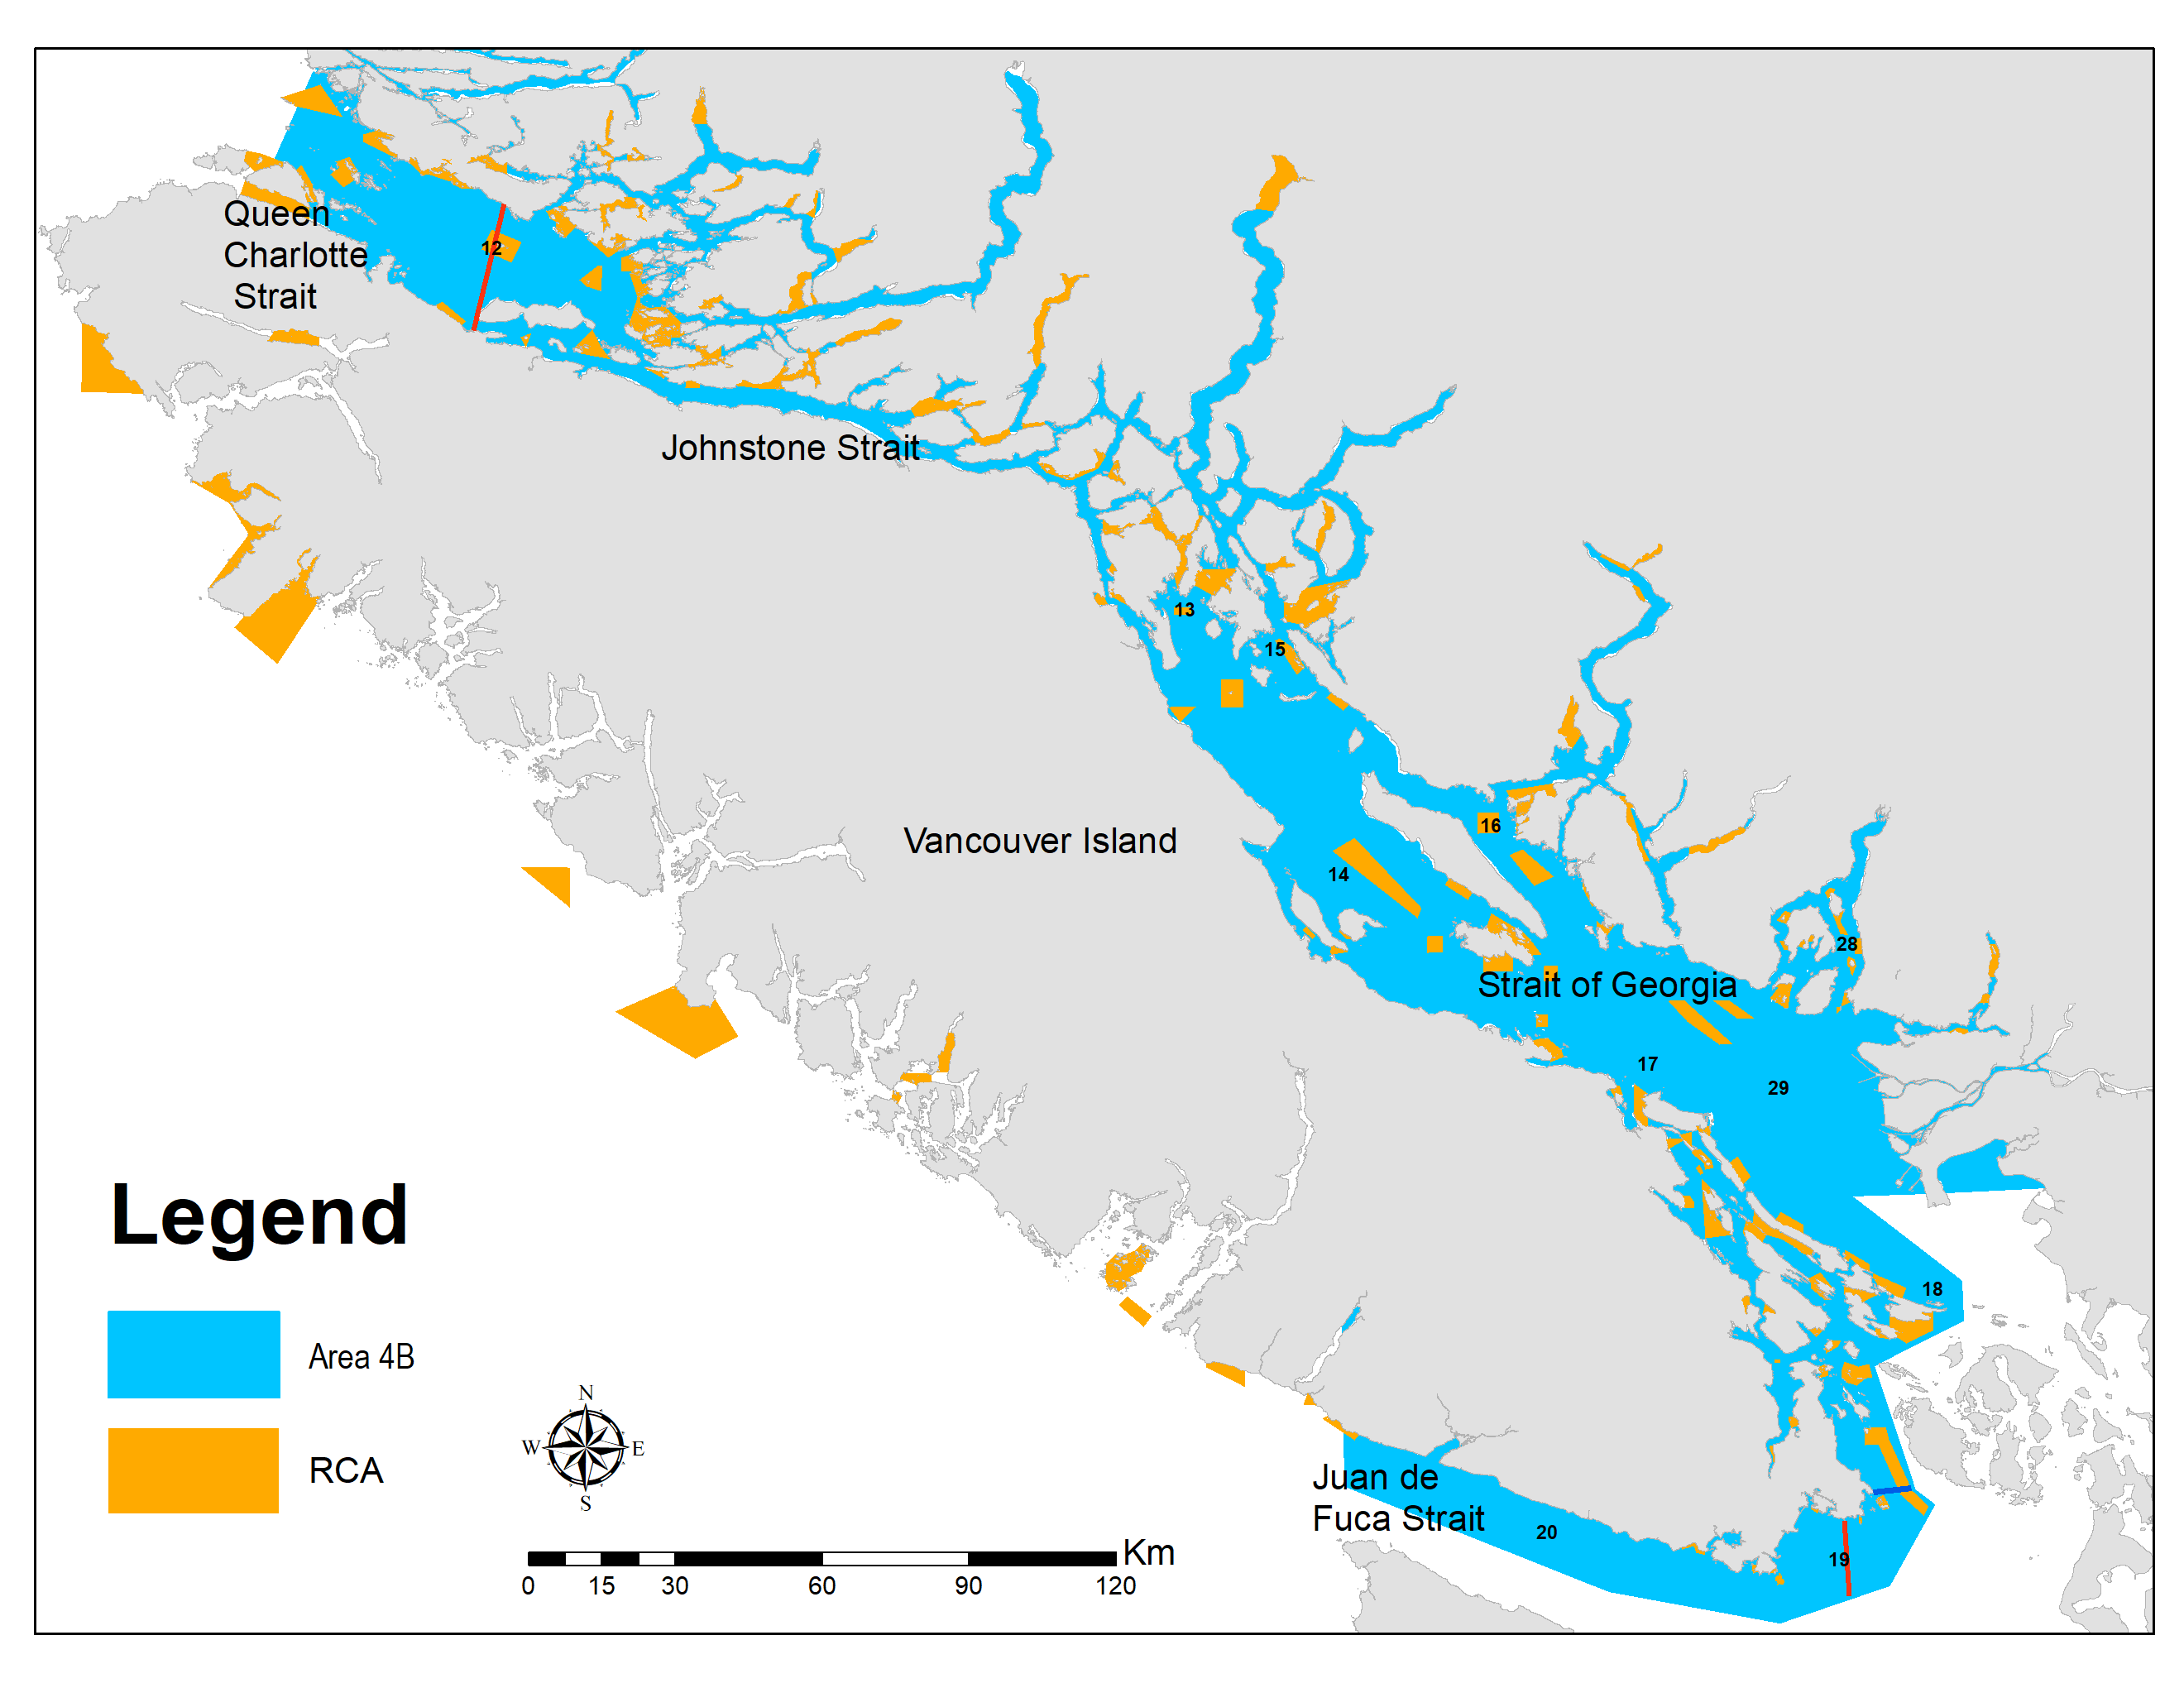
\includegraphics[width=5in]{C:/GitHub/yelloweye-inside/figs/InsideYE_Map_new}}{Figure \ref{fig:map-4B}} 

}

\caption{Map of Groundfish Management Area 4B showing rockfish conservation areas (RCAs) and the boundaries separating the Inside Yelloweye Rockfish designatable unit (DU) from the Outside Yelloweye Rockfish DU. The red lines indicate a proposed adjustment to the range for the Inside DU, based on recent genetic evidence (Siegle \protect\hyperlink{ref-siegle2011}{2011}; Siegle et al. \protect\hyperlink{ref-siegle2013}{2013}; Andrews et al. \protect\hyperlink{ref-andrews2018}{2018}).}\label{fig:map-4B}
\end{figure}
The current rebuilding plan objective is to ``rebuild the stock above the LRP over 80 years with 56\% probability of success''. The milestone objective is to ``achieve positive trends within each 10 year period''. The current MP for Inside Yelloweye Rockfish aims to keep the total annual catch (commercial, recreational, First Nations food, social and ceremonial (FSC), and survey) below 15 tonnes (see Appendix 9 of DFO (\protect\hyperlink{ref-ifmp2018}{2018}) for details).

The guidance for rebuilding plans in Canada states that there should be a high probability of rebuilding fish stocks out of the critical zone within the stated time-frame (DFO \protect\hyperlink{ref-dfo2013}{2013}). Part of the motivation for this project was concern, expressed by fisheries managers, that the 56\% probability of success stated in the current rebuilding plan (DFO \protect\hyperlink{ref-ifmp2018}{2018}) is inconsistent with the definition of high probability.

The guidance document also identifies some recommended management measures, which include: keeping removals from all sources to the lowest possible level; development of a harvest control rule (HCR); and application of management strategy evaluation (MSE) to evaluate, via simulation, the performance of alternative management measures with respect to meeting rebuilding objectives for the stock (DFO \protect\hyperlink{ref-dfo2013}{2013}). The current rebuilding plan implements an annual fixed total allowable catch (TAC) of 15 metric tonnes (DFO \protect\hyperlink{ref-ifmp2018}{2018}), which has not been simulation-tested.

Yelloweye Rockfish are a long-lived species (up to 121 years in B.C., Keppel and Olsen \protect\hyperlink{ref-keppel2019}{2019}), occurring in rocky demersal habitats that have a patchy, discontinuous distribution along BC's inner coast (Yamanaka et al. \protect\hyperlink{ref-yamanaka2011}{2011}). These life history traits make the species vulnerable to overexploitation by fisheries. The inside stock is considered to be data-limited, as there is sparse availability of age-composition data, a lack of biological data from commercial, recreational, and First Nations' fisheries, and uncertainty in the magnitude of historical catches.

\hypertarget{sec:introduction-mse}{%
\subsection{MANAGEMENT STRATEGY EVALUATION (MSE)}\label{sec:introduction-mse}}

Worldwide, the provision of scientific advice for managing fisheries has been moving towards MSE (or management-oriented) approaches (e.g., Butterworth and Punt \protect\hyperlink{ref-butterworth1999}{1999}; Rademeyer et al. \protect\hyperlink{ref-rademeyer2007}{2007}; Berkson and Thorson \protect\hyperlink{ref-berkson2015}{2015}; Geromont and Butterworth \protect\hyperlink{ref-geromont2015}{2015}; Carruthers et al. \protect\hyperlink{ref-carruthers2016}{2016}; Punt et al. \protect\hyperlink{ref-punt2016}{2016}). MSE focuses on identifying MPs that perform best, with respect to meeting agreed-upon policy and fishery objectives, when implemented in a ``closed-loop'' simulation environment (Figure~\ref{fig:mse-chart-basic}). In output-controlled fisheries, such as the quota-managed BC groundfish fishery, MPs describe management measures for setting catch limits. MPs can vary greatly in their data demands, from very data-rich approaches, including statistical catch-at-age stock assessments with harvest control rules, to simple data rules (``data-limited'' approaches), which only rely on catch data and an index of abundance (e.g., Geromont and Butterworth \protect\hyperlink{ref-geromont2015}{2015}; Carruthers et al. \protect\hyperlink{ref-carruthers2016}{2016}).

Closed-loop simulation is distinguished from conventional stock assessment approaches because it simulates feedback between implementation of MPs and the underlying system (the fish stock and its environment), which is described by one or more operating models (OMs). The closed-loop simulation approach takes into account the effect of the MPs on the system, as well as the future data collected from the system and its use in the MPs (Punt et al. \protect\hyperlink{ref-punt2016}{2016}; Carruthers and Hordyk \protect\hyperlink{ref-carruthers2018}{2018}\protect\hyperlink{ref-carruthers2018}{a}; Anderson et al. \protect\hyperlink{ref-anderson2020gfmp}{2020}\protect\hyperlink{ref-anderson2020gfmp}{a}).


\begin{figure}[htb]

{\centering \pdftooltip{\includegraphics[width=6.3in]{C:/GitHub/yelloweye-inside/figs/mse-chart-simple2}}{Figure \ref{fig:mse-chart-basic}} 

}

\caption{Illustration of the fisheries closed-loop simulation process from Anderson et al. (\protect\hyperlink{ref-anderson2020gfmp}{2020}\protect\hyperlink{ref-anderson2020gfmp}{a}) following Punt et al. (\protect\hyperlink{ref-punt2016}{2016}). The management procedure may be based on a simple data rule (e.g., decrease the allowable catch x\% if the survey index decreases y\%) or it might be an estimation model combined with a harvest control rule.}\label{fig:mse-chart-basic}
\end{figure}
\hypertarget{sec:introduction-approach}{%
\subsection{APPROACH}\label{sec:introduction-approach}}

Data-limitations for the Inside Yelloweye stock pose a challenge to evaluating the expected performance of management measures needed to bring the stock into compliance with the Fish Stocks provisions, i.e., to build the stock out of the critical zone within the agreed time-frame and with the agreed probability. Closed-loop simulation-testing of data-limited MPs allows for evaluation of the relative performance of MPs across a range of uncertainties in, for example, underlying fish biology, observation error, estimation error, and implementation error (e.g., Kell et al. \protect\hyperlink{ref-kell2006}{2006}; Carruthers et al. \protect\hyperlink{ref-carruthers2016}{2016}).

Since 2017, a partnership agreement between the University of British Columbia (UBC) and DFO (DFO \protect\hyperlink{ref-dfo_dlmtool_2017}{2017}) has supported development of two open-source software packages for MSE, implemented in the statistical programming environment R (R Core Team \protect\hyperlink{ref-r2019}{2019}): the Data Limited Methods toolkit (DLMtool) (Carruthers and Hordyk \protect\hyperlink{ref-carruthers2018}{2018}\protect\hyperlink{ref-carruthers2018}{a}, \protect\hyperlink{ref-carruthers_hordyk_2018}{2018}\protect\hyperlink{ref-carruthers_hordyk_2018}{b}) and the Management Strategy Evaluation toolkit (MSEtool) (Huynh et al. \protect\hyperlink{ref-huynh_msetool_2019}{2019}). After several years of development, these packages provide some of the fastest, most flexible and extensible software for conducting MSE for fisheries. They can be applied to data-poor or data-rich stocks, enabling rapid assessment of multiple MPs according to customizable conservation and fisheries objectives, and evaluation of key trade-offs.

\hypertarget{sec:introduction-mp-framework}{%
\subsubsection{The Management Procedure Framework for Groundfish in British Columbia}\label{sec:introduction-mp-framework}}

Concurrently with the development of this document, a management procedure framework (MP Framework) for Groundfish in British Columbia (Anderson et al. \protect\hyperlink{ref-anderson2020gfmp}{2020}\protect\hyperlink{ref-anderson2020gfmp}{a}) has been developed for evaluating performance of a wide range of MPs for data-limited groundfish species. The MP Framework uses the functionality of DLMtool and MSEtool extensively, supported by an R package gfdlm (Anderson et al. \protect\hyperlink{ref-gfdlm}{2020}\protect\hyperlink{ref-gfdlm}{c}) written by the authors of Anderson et al. (\protect\hyperlink{ref-anderson2020gfmp}{2020}\protect\hyperlink{ref-anderson2020gfmp}{a}), which houses a suite of software support tools and custom visualizations.

We follow the MP Framework for selecting MPs to set catch limits for data-limited groundfish stocks (Anderson et al. \protect\hyperlink{ref-anderson2020gfmp}{2020}\protect\hyperlink{ref-anderson2020gfmp}{a}). Our evaluation of the Inside Yelloweye rebuilding plan represents the first application of the MP Framework for providing science advice in support of catch decisions. The framework follows six best practice steps described below and in greater detail in Anderson et al. (\protect\hyperlink{ref-anderson2020gfmp}{2020}\protect\hyperlink{ref-anderson2020gfmp}{a}).

The best practice steps are based on a review by Punt et al. (\protect\hyperlink{ref-punt2016}{2016}), who identified five key steps in the MSE process (Steps 2--6 below). An additional first step of the MP Framework, defining the decision context, was identified by Gregory et al. (\protect\hyperlink{ref-gregory2012}{2012}) and Cox and Benson (\protect\hyperlink{ref-cox2016}{2016}). In large part, the DLMtool software has been designed to allow practitioners to follow these steps (Figure~\ref{fig:mse-chart}; Carruthers and Hordyk \protect\hyperlink{ref-carruthers2018}{2018}\protect\hyperlink{ref-carruthers2018}{a}).


\begin{figure}[htb]

{\centering \pdftooltip{\includegraphics[width=\textwidth]{C:/GitHub/yelloweye-inside/figs/mse-chart}}{Figure \ref{fig:mse-chart}} 

}

\caption{The steps of the MSE process following Punt et al. (\protect\hyperlink{ref-punt2016}{2016}) as implemented in DLMtool. Copied from Anderson et al. (\protect\hyperlink{ref-anderson2020gfmp}{2020}\protect\hyperlink{ref-anderson2020gfmp}{a}) and adapted from Carruthers and Hordyk (\protect\hyperlink{ref-carruthers2018}{2018}\protect\hyperlink{ref-carruthers2018}{a}). This figure expands on Figure~\ref{fig:mse-chart-basic}.}\label{fig:mse-chart}
\end{figure}
The six steps are as follows:

Step 1: Definition of the decision context.

Step 2: Selection of objectives and performance metrics.

Step 3: Selection of uncertainties/specification of operating models.

Step 4: Identification of candidate management procedures.

Step 5: Simulation of the application of the management procedures.

Step 6: Presentation of results and selection of management procedure.

After selection and implementation of the MP for setting the catch limit (Figure~\ref{fig:mse-chart}; e.g., applying the selected MP algorithm to the observed survey index), a final necessary step is to periodically monitor and evaluate the performance of the MP (DFO \protect\hyperlink{ref-dfo2013}{2013}; Dowling et al. \protect\hyperlink{ref-dowling2015a}{2015}; Carruthers and Hordyk \protect\hyperlink{ref-carruthers2018}{2018}\protect\hyperlink{ref-carruthers2018}{a}). This may be done through informal means, e.g., via feedback from fishers and survey information (e.g., Cox and Kronlund \protect\hyperlink{ref-cox2008a}{2008}), or through more formal statistical measures, where observed data are compared to predictions from the OMs to test whether the system is performing as expected (Butterworth \protect\hyperlink{ref-butterworth2008}{2008}; Carruthers and Hordyk \protect\hyperlink{ref-carruthers_hordyk_2018}{2018}\protect\hyperlink{ref-carruthers_hordyk_2018}{b}; discussed in Anderson et al. \protect\hyperlink{ref-anderson2020gfmp}{2020}\protect\hyperlink{ref-anderson2020gfmp}{a}).

In the following sections, we describe our approach for developing a candidate rebuilding plan for Inside Yelloweye Rockfish, following the six best practice steps.

\hypertarget{computational-environment}{%
\section{COMPUTATIONAL ENVIRONMENT}\label{computational-environment}}

This version of the document was generated on 2021-05-27 15:53:34 with R version 3.6.3 (2020-02-29) (R Core Team \protect\hyperlink{ref-r2019}{2019}) and R package versions:
\begin{longtable}[]{@{}lll@{}}
\toprule
Package & Version & Date\tabularnewline
\midrule
\endhead
bookdown & 0.17 & 2020-01-11\tabularnewline
cowplot & 1.0.0 & 2019-07-11\tabularnewline
csasdown & 0.0.10.9000 & 2021-05-25\tabularnewline
DLMtool & 5.4.1 & 2019-12-06\tabularnewline
dplyr & 0.8.4 & 2020-01-31\tabularnewline
gfdata & 0.0.0.9000 & 2020-03-04\tabularnewline
gfdlm & 0.0.1.9000 & 2020-03-26\tabularnewline
gfplot & 0.1.4 & 2019-12-10\tabularnewline
ggplot2 & 3.2.1 & 2019-08-10\tabularnewline
knitr & 1.28 & 2020-02-06\tabularnewline
MSEtool & 1.4.3 & 2020-01-10\tabularnewline
purrr & 0.3.3 & 2019-10-18\tabularnewline
rmarkdown & 2.1 & 2020-01-20\tabularnewline
tidyr & 1.0.2 & 2020-01-24\tabularnewline
TMB & 1.7.16 & 2020-01-15\tabularnewline
\bottomrule
\end{longtable}
The source code for this document is available at:\\
\url{https://github.com/pbs-assess/yelloweye-inside/tree/2f9a8a4}.

This document was compiled with the R package csasdown (Anderson et al. \protect\hyperlink{ref-csasdown}{2020}\protect\hyperlink{ref-csasdown}{b}).

The specific versions of the primary packages used to generate this report can be viewed at:

\url{https://github.com/DLMtool/DLMtool/tree/fa971cf}\\
\url{https://github.com/tcarruth/MSEtool/tree/fa1498c}~\\
\url{https://github.com/pbs-assess/gfdata/tree/7292039}~\\
\url{https://github.com/pbs-assess/gfplot/tree/e0b36c0}~\\
\url{https://github.com/pbs-assess/gfdlm/tree/b895686}~\\
\url{https://github.com/pbs-assess/csasdown/tree/f9d5081}~\\

\vspace{4mm}

or installed via:

\texttt{\#\ install.packages(\textquotesingle{}devtools\textquotesingle{})}\\
\texttt{devtools::install\_github(\textquotesingle{}DLMtool/DLMtool\textquotesingle{},\ ref\ =\ \textquotesingle{}fa971cf\textquotesingle{})}~\\
\texttt{devtools::install\_github(\textquotesingle{}tcarruth/MSEtool\textquotesingle{},\ ref\ =\ \textquotesingle{}fa1498c\textquotesingle{})}~\\
\texttt{devtools::install\_github(\textquotesingle{}pbs-assess/gfdata\textquotesingle{},\ ref\ =\ \textquotesingle{}7292039\textquotesingle{})}~\\
\texttt{devtools::install\_github(\textquotesingle{}pbs-assess/sha\_gfplot\textquotesingle{},\ ref\ =\ \textquotesingle{}e0b36c0\textquotesingle{})}~\\
\texttt{devtools::install\_github(\textquotesingle{}pbs-assess/gfdlm\textquotesingle{},\ ref\ =\ \textquotesingle{}b895686\textquotesingle{})}~\\
\texttt{devtools::install\_github(\textquotesingle{}pbs-assess/csasdown\textquotesingle{},\ ref\ =\ \textquotesingle{}f9d5081\textquotesingle{})}~\\

\clearpage

\hypertarget{refs}{}
\leavevmode\hypertarget{ref-anderson2020gfmp}{}%
Anderson, S.C., Forrest, R.E., Huynh, Q.C., and Keppel, E.A. 2020a. A management procedure framework for groundfish in British Columbia. DFO Can. Sci. Advis. Sec. Res. Doc. 2020/nnn: In prep.

\leavevmode\hypertarget{ref-csasdown}{}%
Anderson, S.C., Grandin, C., Edwards, A.M., Grinnell, M.H., Ricard, D., and Haigh, R. 2020b. csasdown: Reproducible CSAS reports with bookdown. R package version 0.0.8. \url{https://github.com/pbs-assess/csasdown}.

\leavevmode\hypertarget{ref-gfdlm}{}%
Anderson, S.C., Grandin, C., and Forrest, R.E. 2020c. gfdlm: Tools for working with DLMtool and MSEtool. R package version 0.0.1.9000. \url{https://github.com/pbs-assess/gfdlm}.

\leavevmode\hypertarget{ref-andrews2018}{}%
Andrews, K.S., Nichols, K.M., Elz, A., Tolimieri, N., Harvey, C.J., Pacunski, R., Lowry, D., Yamanaka, K.L., and Tonnes, D.M. 2018. Cooperative research sheds light on population structure and listing status of threatened and endangered rockfish species. Conserv. Genet. 19(4): 865--878.

\leavevmode\hypertarget{ref-berkson2015}{}%
Berkson, J., and Thorson, J.T. 2015. The determination of data-poor catch limits in the United States: Is there a better way? ICES J. Mar. Sci. 72(1): 237--242.

\leavevmode\hypertarget{ref-butterworth2008}{}%
Butterworth, D.S. 2008. Some lessons from implementing management procedures. Edited by K. Tsukamoto, T. Kawamura, T. Takeuchi, T.D. Beard, Jr., And M.J. Kaiser. \emph{In} Fisheries for Global Welfare and Environment, 5th World Fisheries Congress 2008. TERRAPUB, Toyko. pp. 381--397.

\leavevmode\hypertarget{ref-butterworth1999}{}%
Butterworth, D.S., and Punt, A.E. 1999. Experiences in the evaluation and implementation of management procedures. ICES J. Mar. Sci. 56(6): 985--998.

\leavevmode\hypertarget{ref-carruthers2018}{}%
Carruthers, T.R., and Hordyk, A. 2018a. The data-limited methods toolkit (DLMtool): An R package for informing management of data-limited populations. Methods Ecol. Evol. 9: 2388--2395.

\leavevmode\hypertarget{ref-carruthers_hordyk_2018}{}%
Carruthers, T.R., and Hordyk, A.R. 2018b. Using management strategy evaluation to establish indicators of changing fisheries. Can. J. Fish. Aquat. Sci.: 1--16.

\leavevmode\hypertarget{ref-carruthers2016}{}%
Carruthers, T.R., Kell, L.T., Butterworth, D.D.S., Maunder, M.N., Geromont, H.F., Walters, C., McAllister, M.K., Hillary, R., Levontin, P., Kitakado, T., and Davies, C.R. 2016. Performance review of simple management procedures. ICES J. Mar. Sci. J. Cons. 73(2): 464--482.

\leavevmode\hypertarget{ref-cosewic2008}{}%
COSEWIC. 2008. COSEWIC assessment and status report on the Yelloweye Rockfish (\emph{Sebastes ruberrimus}), Pacific Ocean inside waters population and Pacific Ocean outside waters population, in Canada. Committee on the Status of Endangered Wildlife in Canada \url{https://www.sararegistry.gc.ca/virtual_sara/files/cosewic/sr_yelloweye_rockfish_0809_e.pdf}.

\leavevmode\hypertarget{ref-cox2016}{}%
Cox, S.P., and Benson, A.J. 2016. Roadmap to more sustainable Pacific herring fisheries in Canada: A step-by-step guide to the management strategy evaluation approach.

\leavevmode\hypertarget{ref-cox2008a}{}%
Cox, S.P., and Kronlund, A.R. 2008. Practical stakeholder-driven harvest policies for groundfish fisheries in British Columbia, Canada. Fish. Res. 94(3): 224--237.

\leavevmode\hypertarget{ref-dfo2006}{}%
DFO. 2006. A harvest strategy compliant with the Precautionary Approach. DFO Can. Sci. Advis. Sec. Sci. Advis. Rep. 2006/023.

\leavevmode\hypertarget{ref-dfo2009}{}%
DFO. 2009. A fishery decision-making framework incorporating the Precautionary Approach \url{https://www.dfo-mpo.gc.ca/reports-rapports/regs/sff-cpd/precaution-back-fiche-eng.htm}.

\leavevmode\hypertarget{ref-dfo2012}{}%
DFO. 2012. Survey of recreational fishing in canada 2010. DFO Res. Manage. Eco. Fish. Manage. 2012-1804.

\leavevmode\hypertarget{ref-dfo2013}{}%
DFO. 2013. Guidance for the development of rebuilding plans under the Precautionary Approach framework~: Growing stocks out of the critical zone \url{https://www.dfo-mpo.gc.ca/reports-rapports/regs/sff-cpd/precautionary-precaution-eng.htm}.

\leavevmode\hypertarget{ref-dfo_dlmtool_2017}{}%
DFO. 2017. DLMtool phase II: Developing a management strategy evaluation package for advancing the science and management of data-limited and at-risk Canadian fish stocks. PAC2016.12 \url{https://www.dfo-mpo.gc.ca/science/collaboration/partnershipprojects/\%0A\%20\%20\%20\%20\%20\%20\%20\%20\%20\%20\%20\%20\%20\%20\%20\%20\%20\%20005-eng.html}.

\leavevmode\hypertarget{ref-ifmp2018}{}%
DFO. 2018. Pacific Region integrated fisheries management plan, groundfish, effective February 21, 2018 \url{http://waves-vagues.dfo-mpo.gc.ca/Library/40657814.pdf}.

\leavevmode\hypertarget{ref-dowling2015a}{}%
Dowling, N.A., Dichmont, C.M., Haddon, M., Smith, D.C., Smith, A.D., and Sainsbury, K. 2015. Guidelines for developing formal harvest strategies for data-poor species and fisheries. Fish. Res. 171: 130--140.

\leavevmode\hypertarget{ref-geromont2015}{}%
Geromont, H.F., and Butterworth, D.S. 2015. Complex assessments or simple management procedures for efficient fisheries management: A comparative study. ICES J. Mar. Sci. 72(1): 262--274.

\leavevmode\hypertarget{ref-gregory2012}{}%
Gregory, R., Failing, L., Harstone, M., Long, G., and McDaniels, T.L. (\emph{Editors}). 2012. Structured decision making: A practical guide to environmental management choices. Wiley-Blackwell, Oxford.

\leavevmode\hypertarget{ref-huynh_msetool_2019}{}%
Huynh, Q.C., Hordyk, A.R., and Carruthers, T. 2019. MSEtool: Management strategy evaluation toolkit. R package version 1.4.3.

\leavevmode\hypertarget{ref-kell2006}{}%
Kell, L.T., De Oliveira, J.A.A., Punt, A.E., McAllister, M.K., and Kuikka, S. 2006. Chapter 15 Operational management procedures: An introduction to the use of evaluation frameworks. Dev. Aquacult. Fish. Sci. 36: 379--407.

\leavevmode\hypertarget{ref-keppel2019}{}%
Keppel, E.A., and Olsen, N. 2019. Pre-COSEWIC review of Yelloweye Rockfish (\emph{Sebastes ruberrimus}) along the Pacific coast of Canada: Biology, distribution and abundance trends. DFO Can. Sci. Advis. Sec. Res. Doc 2019/014.

\leavevmode\hypertarget{ref-punt2016}{}%
Punt, A.E., Butterworth, D.S., de Moor, C.L., De Oliveira, J.A.A., and Haddon, M. 2016. Management strategy evaluation: Best practices. Fish Fish. 17(2): 303--334.

\leavevmode\hypertarget{ref-rademeyer2007}{}%
Rademeyer, R.A., Plagányi, É.E., and Butterworth, D.S. 2007. Tips and tricks in designing management procedures. ICES J. Mar. Sci. 64(4): 618--625.

\leavevmode\hypertarget{ref-r2019}{}%
R Core Team. 2019. R: A language and environment for statistical computing. R Foundation for Statistical Computing, Vienna, Austria.

\leavevmode\hypertarget{ref-siegle2011}{}%
Siegle, M.R. 2011. Population structure in yelloweye rockfish (\emph{Sebastes ruberrimus}) driven by limited dispersal and selection. Thesis.

\leavevmode\hypertarget{ref-siegle2013}{}%
Siegle, M.R., Taylor, E.B., Miller, K.M., Withler, R.E., and Yamanaka, K.L. 2013. Subtle population genetic structure in Yelloweye Rockfish (\emph{Sebastes ruberrimus}) is consistent with a major oceanographic division in British Columbia, Canada. PLoS ONE 8(8): e71083.

\leavevmode\hypertarget{ref-yamanaka2011}{}%
Yamanaka, K.L., McAllister, M.K., Olesiuk, P.F., Etienne, M.-P., Obradovich, S.G., and Haigh, R. 2011. Stock assessment for the inside population of Yelloweye Rockfish (\emph{Sebastes ruberrimus}) for British Columbia, Canada for 2010. DFO Can. Sci. Advis. Sec. Res. Doc. 2011/129. xiv + 131 p.

\end{document}
